%% This is an example first chapter.  You should put chapter/appendix that you
%% write into a separate file, and add a line \include{yourfilename} to
%% main.tex, where `yourfilename.tex' is the name of the chapter/appendix file.
%% You can process specific files by typing their names in at the 
%% \files=
%% prompt when you run the file main.tex through LaTeX.
\chapter{Overview of Visual-inertial Odometry}
\label{chap:Overview}

In this chapter, we will overview visual-inertial odometry system. In section \ref{sec:notations}, we will introduce world representation(\eg, world frame, camera frame and IMU frame) together with basic notations in our odometry system. Then in section \ref{sec:FVK}, we will discuss two important scheme, filter method and keyframe Bundle Adjustment(keyframe BA) in SLAM algorithm, and explain why we finally choose keyframe-based method.

\section{World Representations and Notations}
\label{sec:notations}

\begin{figure}[h]
    \centering
    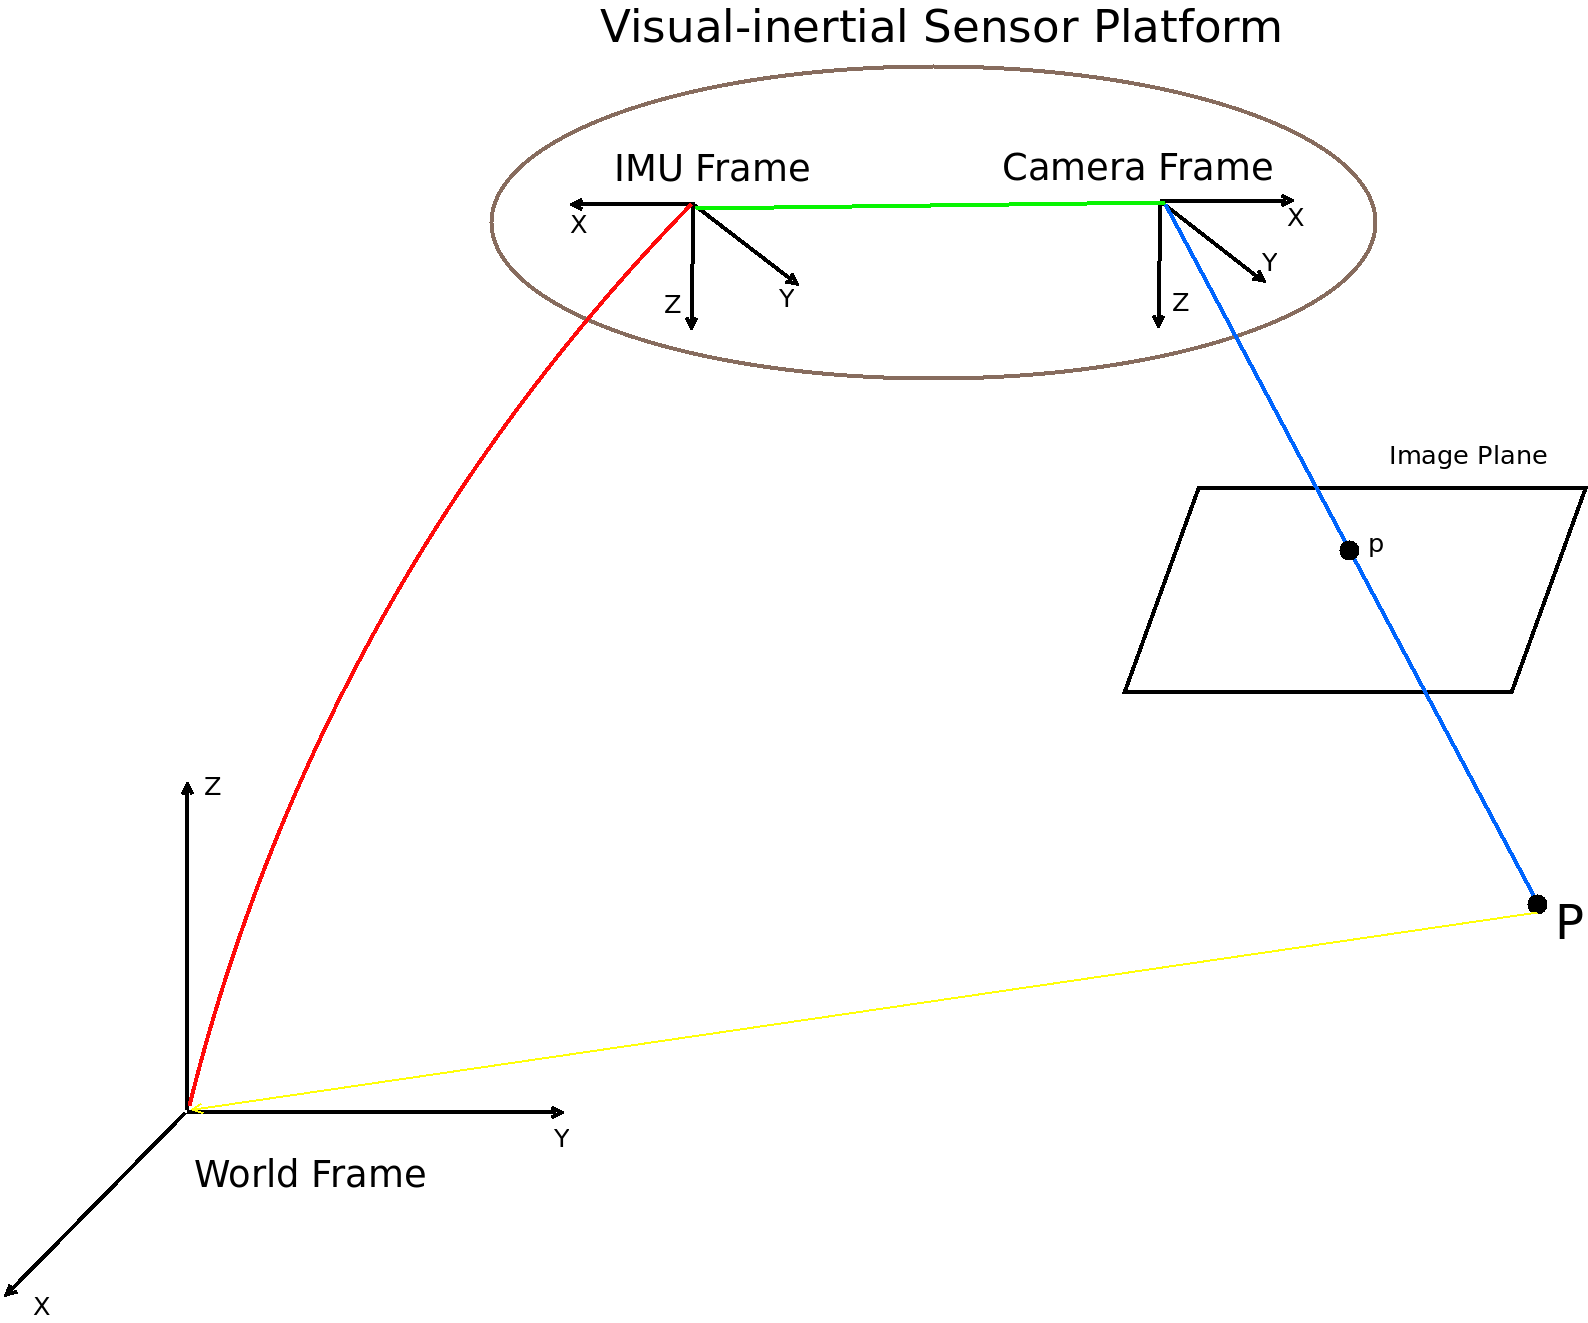
\includegraphics[width=0.8\textwidth]{CONTENT/Figure/Figure2-1_World.png}
    \caption{This figure shows the connection among world frame $\W$, IMU frame $\I$ and camera frame $\C$. Green line shows the transformation between camera and IMU, which can be pre-calibrated. Red line is the pose of IMU in world frame. Camera frame observes point $\textbf{p}$ of object P in image plane, and connects a object P by blue line, and the coordinate of object P in world frame is presented as yellow line.}
    \label{fig:fig2-1}
\end{figure}

Visual-inertial odometry~\cite{li2011consistency}, literally, is an odometry system, which received environment information by visual (camera) and inertial (IMU) sensor. VIO is similar with well-known visual odometry (VO) problem \cite{nister2004visual}, with an additional IMU sensor, it tries to estimate agent's pose as agent keep moving in the environment. One big difference between VIO and SLAM algorithm is that VIO does not or only build a simple map, whereas SLAM normally maintains and continuously updates a map.

To setup a VIO system, we need to first define the ways to represent the world. Globally, we have a world frame $\W$; World frame $\W$ is set to a right-handed Cartesian coordinate system that every objects has an absolute pose (translation and rotation) in it. Then we have local frame for each sensor, \ie, IMU frame $\I$ and camera frame $\C$; Every time camera and IMU sensor obtain observations within their own local frame, we need to integrate those data and estimate the pose of those sensors in world frame $\W$. Figure \ref{fig:fig2-1} shows the overall world representations. Both IMU frame and Camera frame are right-handed Cartesian coordinate system.

In this master thesis, we use following notations,
\begin{itemize}
\item {We denote scalars as $a, b, c$, vectors as $\textbf{a}, \textbf{b}, \textbf{c}$, matrices as $\mA, \mB, \mC$, frames as $\A, \B, \C$.}
\item {We denote measurement $\textbf{m}$ in particular frame $\F$ as $\textbf{m}_{\F}$. To further simplify, any parameter that is \textbf{not} in world frame shall 
be denoted particularly. For example, the translation $\textbf{p}$ in camera frame will be denoted as $\textbf{p}_{\C}$, and the translation $\textbf{p}$ in world frame will be denoted as $\textbf{p}$. }
\item {A general translation $\textbf{t}$ should express a translation from point $A$ to point $B$ in frame $\C$, which is denoted as $\textbf{t}^{AB}_{\C}$. We simplify a point $\textbf{p}$ in frame $\A$ as $\textbf{p}_{\A}$, when this point is the translation $\textbf{t}^{OP}_{\A}$, $O$ is origin of frame $\A$, and $\textbf{p} = P$, this holds same for vector.}
\item {A general rotation is either expressed in quaternion $\textbf{q}$ or rotation matrix $\mR$. We use quaternion $\textbf{q}$ as example. A quaternion is a  orientation operation from frame $\B$ to frame $\A$, and it is denoted as $\textbf{q}_{\A\B}$  in this thesis. Noted that if such a operation is from world frame $\W$ to some frame $\B$, we omit both frame for simplification, \ie, $\textbf{q}_{\W\B} \triangleq \textbf{q}$.}
%TODO: Add more notations when necessary
\end{itemize}

\section{Filter Versus Keyframe}
\label{sec:FVK}

\begin{figure}
\centering
	\begin{subfloat}[Filter]{
		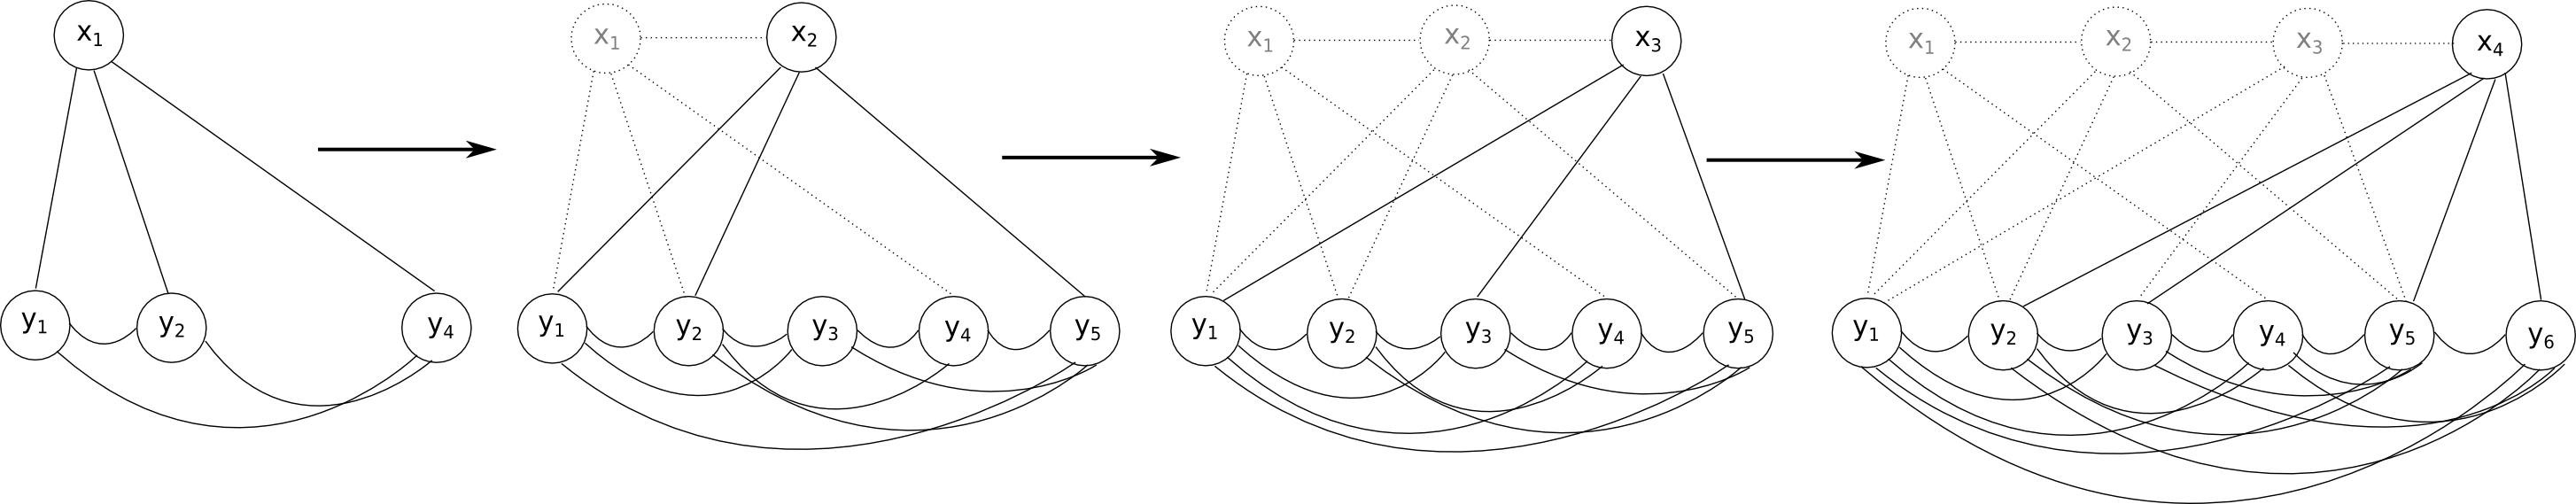
\includegraphics[width=0.8\textwidth]{CONTENT/Figure/Figure2-2-a.png}
		\label{fig:fig2-2-a}}
	\end{subfloat}
	
	%\hspace*{\fill} % separation between the subfigures
	
	\begin{subfloat}[Keyframe-based BA]{
		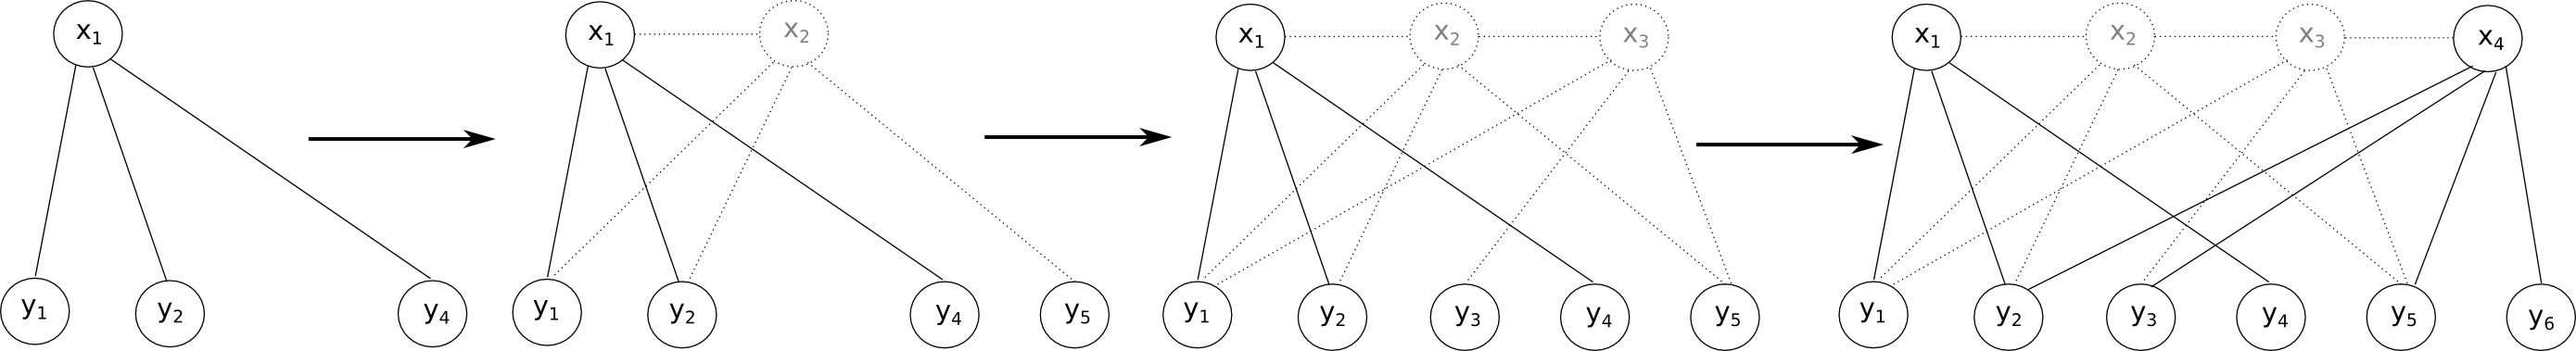
\includegraphics[width=0.8\textwidth]{CONTENT/Figure/Figure2-2-b.png}
		\label{fig:fig2-2-b}}
	\end{subfloat}
	
	%\hspace*{\fill} % separation between the subfigures
	
	\caption{(a) Filter method for SLAM. (b) Keyframe-based Bundle Adjustment (BA) for SLAM. We denote the $i^{th}$ camera position as $\textbf{x}_i$,  $i^{th}$ image feature as $\textbf{y}_i$. We connect the line between camera and image feature if this feature is observed by this camera, the vanished observations is presented as dotted line, and the vanished camera is expressed as grey font. Both graph changes as time goes on from left to right. One can see from (a) that though only the latest camera pose is reserved, the edges between features are increasing exponentially. (b) stores some of former camera poses (keyframe) (\ie, $\textbf{x}_1$ and $\textbf{x}_4$) by keeping graph stay sparsity. } 
	\label{fig:fig2-2}
\end{figure}

It is important to note that though this thesis focus on visual-inertial odometry for small workspace, we still tend to keep the possibility to extend our system to a general, scalable and efficient SLAM system. SLAM system usually have two parallel process, one is for localization and the other is for mapping, the crucial point of building such a system is to keep both processes efficient. There are two general framework (\eg, filter-based method and keyframe-based method) in SLAM. In this section, we want to discuss whether filter-based method or keyframe-based method are more suitable for our case.

Filter-based SLAM \cite{davison2007monoslam, eade2007monocular, davison2003real} uses \textit{Extended Kalman Filter} (EKF) to propagate state and update the covariance of the state. In each step, system obtain the current pose estimation and map update by marginalising all former information. This marginalising step usually eliminates the former pose and adds connections to image features. As showed in Figure~\ref{fig:fig2-2-a}, the graph will not grow fast with time since the former pose has been eliminated and features in environment is limited. However, once the system moves to large scale scene, the problem of limiting the number of features become severe as the graph tends to be fully-connected. 
   
Keyframe-based SLAM \cite{klein2007parallel, mourikis2007multi, forster2014svo, engel2014lsd, mur2015orb} applies \textit{bundle adjustment} (BA) for keyframes to update the map in each step. In keyframe-based SLAM, it stores some historical poses (keyframes), and combines with image feature points to do a BA step. The chosen of keyframes varies from implementations, the idea is to pick up the poses that is not very close to last keyframe, otherwise the information might be redundant, which might lead to increase the computational cost. In Figure~\ref{fig:fig2-2-b}, the graph still stays sparsity as the number of poses and features increases. The drawback might be the behaviour of pose estimation is inadequate as it ignores some of former information.

In \cite{strasdat2010real}, they conclude that keyframe-based SLAM is slightly better than filter-based SLAM in their experiment settings, especially when scale of scene becomes larger. In this master thesis, we choose keyframe-based method for visual part and filter method for IMU integration part. We choose filter method for IMU integration part is that we do not keep former information (\eg, image features or landmarks) in integration step, hence each filter step can be regarded as an optimization step. The reason why we use keyframe-based method for visual part is that we want keep the scalability of our system, besides the results from IMU integration can be a good compensation in case of the lack of pose estimation in keyframe-based BA.

